\documentclass[11pt,a4paper,oneside]{article}\usepackage[]{graphicx}\usepackage[]{color}
%% maxwidth is the original width if it is less than linewidth
%% otherwise use linewidth (to make sure the graphics do not exceed the margin)
\makeatletter
\def\maxwidth{ %
  \ifdim\Gin@nat@width>\linewidth
    \linewidth
  \else
    \Gin@nat@width
  \fi
}
\makeatother

\definecolor{fgcolor}{rgb}{0.345, 0.345, 0.345}
\newcommand{\hlnum}[1]{\textcolor[rgb]{0.686,0.059,0.569}{#1}}%
\newcommand{\hlstr}[1]{\textcolor[rgb]{0.192,0.494,0.8}{#1}}%
\newcommand{\hlcom}[1]{\textcolor[rgb]{0.678,0.584,0.686}{\textit{#1}}}%
\newcommand{\hlopt}[1]{\textcolor[rgb]{0,0,0}{#1}}%
\newcommand{\hlstd}[1]{\textcolor[rgb]{0.345,0.345,0.345}{#1}}%
\newcommand{\hlkwa}[1]{\textcolor[rgb]{0.161,0.373,0.58}{\textbf{#1}}}%
\newcommand{\hlkwb}[1]{\textcolor[rgb]{0.69,0.353,0.396}{#1}}%
\newcommand{\hlkwc}[1]{\textcolor[rgb]{0.333,0.667,0.333}{#1}}%
\newcommand{\hlkwd}[1]{\textcolor[rgb]{0.737,0.353,0.396}{\textbf{#1}}}%
\let\hlipl\hlkwb

\usepackage{framed}
\makeatletter
\newenvironment{kframe}{%
 \def\at@end@of@kframe{}%
 \ifinner\ifhmode%
  \def\at@end@of@kframe{\end{minipage}}%
  \begin{minipage}{\columnwidth}%
 \fi\fi%
 \def\FrameCommand##1{\hskip\@totalleftmargin \hskip-\fboxsep
 \colorbox{shadecolor}{##1}\hskip-\fboxsep
     % There is no \\@totalrightmargin, so:
     \hskip-\linewidth \hskip-\@totalleftmargin \hskip\columnwidth}%
 \MakeFramed {\advance\hsize-\width
   \@totalleftmargin\z@ \linewidth\hsize
   \@setminipage}}%
 {\par\unskip\endMakeFramed%
 \at@end@of@kframe}
\makeatother

\definecolor{shadecolor}{rgb}{.97, .97, .97}
\definecolor{messagecolor}{rgb}{0, 0, 0}
\definecolor{warningcolor}{rgb}{1, 0, 1}
\definecolor{errorcolor}{rgb}{1, 0, 0}
\newenvironment{knitrout}{}{} % an empty environment to be redefined in TeX

\usepackage{alltt}
\usepackage{amsmath,amsthm,amsfonts,amssymb}
\usepackage{pst-eucl,pstricks,pstricks-add,multido, pst-plot}
\usepackage[utf8]{inputenc}
%\usepackage[latin1]{inputenc}
\usepackage[english,activeacute]{babel}
\usepackage[a4paper,margin=2.5cm]{geometry}
\usepackage{times}
\usepackage{mathtools}
\usepackage[T1]{fontenc}
\usepackage{titlesec}
\usepackage{url}
\usepackage{bbm}
\usepackage{enumitem}  
\usepackage{float}
\usepackage{cite}
\usepackage{graphicx}
\usepackage{wrapfig}
\usepackage{lipsum}
\usepackage{multicol}
\usepackage{float}
\usepackage{lmodern}
\usepackage{epstopdf}
\parindent=0mm
\usepackage{color, colortbl}
\definecolor{azul}{rgb}{0.63, 0.79, 0.95}

\newtheorem{thm}{Theorem}[subsection]
\newtheorem{defi}[subsection]{Definition}
\newtheorem{exm}{Example}
\newtheorem{lema}[thm]{Lemma}
\newtheorem{coro}{Corollary}[thm]
\newcommand{\threepartdef}[3]
{
	\left\{
		\begin{array}{ll}
			#1 \\
			#2 \\
			#3 \\
		\end{array}
	\right.
}
\newcommand{\ttwopartdef}[2]
{
	\left\{
		\begin{array}{ll}
			#1 \\
			#2 \\
		\end{array}
	\right.
}

\newcommand*{\titleBOOK}{\begingroup
%\raggedleft
\centering
\vspace*{\baselineskip}
\vspace*{\baselineskip}
{\Huge\scshape Lecture Notes}\\[10mm]
%{\Large \includegraphics[scale=0.25]{uah.pdf}}\\[35mm]
{\Huge\scshape Non Life  \\[5mm]
Insurance} \\ [\baselineskip]
{\Large\bfseries First Draft}\\[0.3 \textheight]
{\Large Prof. Dr. Ricardo Gatto}\\
%{\large\scshape MS-PLUS, Inc.}\par
\vfill
\begin{center}
{\scshape Switzerland-Ecuador}\\
\rule{\textwidth}{0.5pt}
\end{center}
\vspace*{\baselineskip}
\endgroup}
\IfFileExists{upquote.sty}{\usepackage{upquote}}{}
\begin{document}
\titleBOOK
\newpage

\tableofcontents
\newpage


\section{Individual Risk and Distributions}
A non negative random variable is called a \textbf{loss} and it its distribution a \textbf{loss distribution}. One impotant classes of loss distributions are the following\\

$X\sim Exponential(\alpha)$ means that $X$ has density $f_X(x)=\alpha e^{-\alpha x}$ and distribution function (d.f) $F_X(x)=1-e^{-\alpha x}$, $\forall x>0$ and $\alpha>0$.\\

%Pareto Distribution
Let $Y=e^x$, 
\begin{align*}
F_Y(y) &= F_X(\log y)\\
&=1-e^{-\alpha \log (y)}\\
&=1-y^{-\alpha}
\end{align*}
Is called the \textbf{Pareto Distribution}. If $Y$ follows a Pareto distribution, denoted  $Y\sim Pareto(\alpha),\forall y>1$

\begin{knitrout}
\definecolor{shadecolor}{rgb}{0.969, 0.969, 0.969}\color{fgcolor}

{\centering 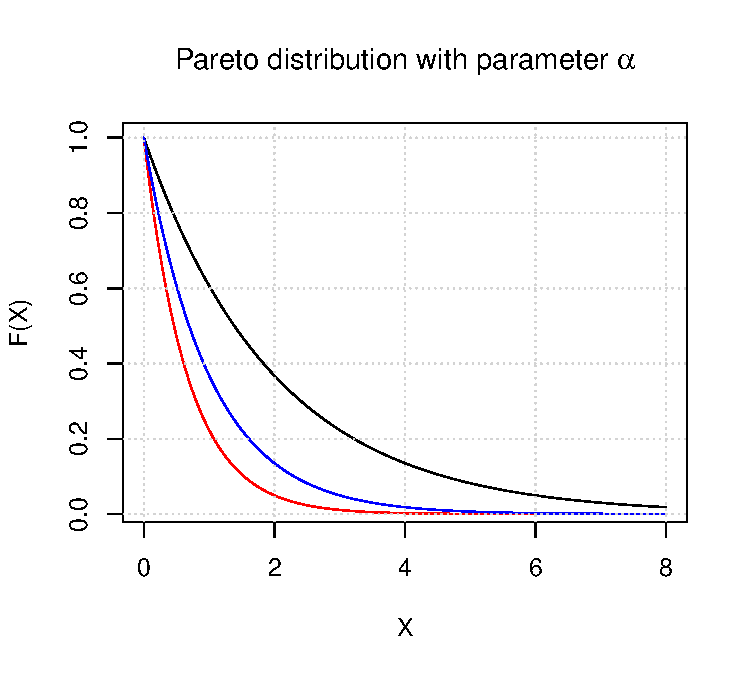
\includegraphics[width=\maxwidth]{figure/unnamed-chunk-1-1} 

}



\end{knitrout}
%Weibull Distribution
$X\sim Exponential (\lambda)$ and $Y\sim X^{\frac{1}{\tau}}$, $\forall \tau>0$
\begin{align*}
F_Y(Y) &= F_X(Y^{\tau})\\
&=1-e^{-\lambda y^{\tau}}, \quad \forall y>0\\
\end{align*}
$Y$ follows the \textbf{Weibull distribution}, $\tau$ is called the Weibull index.\\ It is denoted by $Y\sim Weibull(\tau,\lambda)$

\begin{knitrout}
\definecolor{shadecolor}{rgb}{0.969, 0.969, 0.969}\color{fgcolor}

{\centering 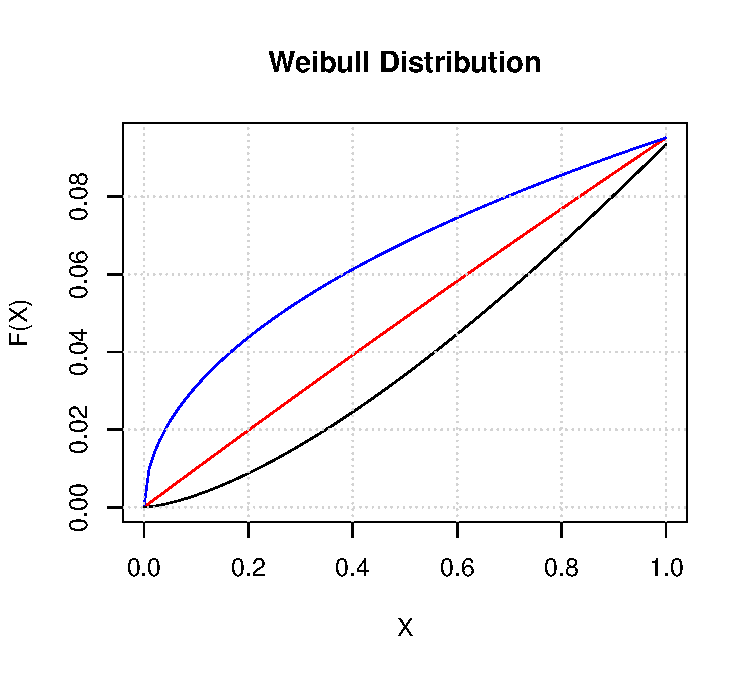
\includegraphics[width=\maxwidth]{figure/unnamed-chunk-2-1} 

}



\end{knitrout}


% Extreme Value Distribution
Let $X\sim Exponential(1)$ and $$Y=\frac{X^{-\gamma}-1}{\gamma} \ \ \ \forall \gamma\neq 0$$

\begin{align*}
F_Y(Y) &= P(Y\leq y)\\
&=P[\frac{X^{-\gamma}-1}{\gamma}\leq Y]\\
&=P[X\geq (1+\gamma x)^{-\frac{1}{\gamma}}]\\
&=1-F_X(\{1+\gamma x\}^{-\frac{1}{\gamma}})\\
&=exp\{-(1+\gamma x)^{-\frac{1}{\gamma}}\}\ \ \ for $1+\gamma x>0$
\end{align*}
 Y follows  the \textbf{Extreme Value Distribution}.
 
 \begin{align*}
 \displaystyle\lim_{\gamma\rightarrow 0}\frac{x^{-\gamma}-1}{\gamma}&=\displaystyle\lim_{\gamma\rightarrow 0}\frac{d}{d\gamma}x^{-\gamma}\\
 &=\displaystyle\lim_{\gamma\rightarrow 0}\frac{d}{d\gamma}e^{-(log x )\gamma}\\
 &=-log x
 \end{align*}

%Gumbel Distribution 
 Let $Y=-log X$, 
 \begin{align*}F_y(y)&=P[-log X\leq Y]\\
 &=P[X\geq e^{-y}]\\
 &=exp\{e^{-y}\} \ \ \forall x\in \mathbb{R}\\
  \end{align*}
$Y$ follows the \textbf{Gumbel} distribution.


%Frechét Distribution
Let $X\sim Exponential(1)$ and $Y=X^{-\frac{1}{\alpha}}$ for $\alpha>0$.
\begin{algin*}
F_Y(y)&=1-F_X(x^{-\alpha})\\
&=1-\{1-e^{-x^{-\alpha}}\}\\
&=exp\{-x^{-\alpha}\}\ \ \ \forall x>0\\
\end{align*}

$Y$ follows the \textbf{Fréchet} Distribution.

%Burr Distribution

$X\sim Pareto(\alpha)$ and $Y=\beta(X-1)$,  $Y=\{\beta(X-1)\}^{\frac{1}{\tau}}$
\begin{align*}for \beta,\tau>0\\
F_Y(y)&=F_x(1+\frac{Y^2}{\beta})\\
\&=1-(1+\frac{Y^2}{\beta})^{-\alpha}\ \ \ \forall y>0 \\
\end{align*}
$Y$ follows the \textbf{Burr} distribution, we denote it as $$Y\sim Burr(\alpha,\beta,\tau)$$


%Lognormal distribution
Let $X\sim \mathcal{N}(\mu,\sigma^2)$ and $Y=e^x$
$$f(y)=\frac{1}{\sqrt{2\pi}\sigma y}exp\{-\frac{1}{2}(\frac{log y-\mu}{\sigma})^2\}\ \ \ \forall y>0$$ $Y$ follows the \textbf{Lognormal} Distribution.
$$Y\sim Lognormal(\mu,\sigma^2)$$

%LogGamma Distribution
Let $X\sim Gamma(\alpha,\beta)$ and $Y=e^x$
$$f_x(x)=\frac{\beta^{\alpha}}{\Gamma(\alpha)}x^{\alpha-1}e^{-\beta x}\ \ \ \forall x>0  \ \ and \ \ \alpha,\beta>0$$ 
$$f_y(y)=\frac{\beta^{\alpha}}{\Gamma(\alpha)}(log y)^{\alpha-1}y^{-\beta-1}\ \ \ \forall y>1 $$
$Y$ follows the log-gamma distribution.
$$Y\sim \textbf{log-gamma}(\alpha,\beta)$$

Let $X\sim\mathcal{N}(0,1)$ and $Y=|X|$
\begin{align*}
F_Y(X)&=P[|X|\leq Y]\\
&=2\phi (y)-1\ \ \forall y>0
\end{align*}

Where $\phi$ is the distribution function $\mathcal{N}(0,1)$
\begin{defi}The distribution function $F_1$ has $\threepartdef{heavier}{equivalent}{lighter}$  right tail as the distribution function $F_2$ if 
$$\displaystyle\lim_{x\rightarrow\infty}\frac{1-F_1(x)}{1-F_2(x)}\threepartdef{>}{=}{<} 1.$$
\end{defi}
\begin{exm}F_1 \  Pareto,\ \ F_2 \ Burr\\
&=\displaystyle\lim_{x\rightarrow\infty}\frac{x^{-\alpha}}{\left(\frac{\beta}{\beta+x^\tau}\right)^{\alpha}}\\
&=\left(\displaystyle\lim_{x\rightarrow\infty}\frac{\beta+x^{\tau}}{\beta x}\right)^{\alpha}\\
&=\left(\frac{1}{\beta}\displaystyle\lim_{x\rightarrow\infty}x^{\tau-1}\right)^{\alpha}=\threepartdef{\infty \hspace{20pt} if \hspace{20pt}\tau>1}{\beta^{-\alpha}\hspace{12pt} if \hspace{20pt} \tau=1}{0 \hspace{25pt}if \hspace{20pt} \tau<1}\\
\end{exm}

\begin{defi}Moments\\
\begin{align*}
E(X^k)&=\displaystyle\int_0^\infty x^kdF(x)\\
&=\displaystyle\int_0^\infty x^k f(x)dx
\end{align*}
\end{Defi}
The existence of moments is a practical problem with heavy tailed distributions.


\begin{lema}
For any (real-valued) random variable $X$.

\item{i. } E[|X|]=\displaystyle\int_0^{\infty}P[|X|>x]dx\\
\item{ii.} E[|X|]<\infty\Rightarrow P[|X|>x]=o(x^{-1})\\

\end{lema}

\begin{proof}
Let G be the d.f of |X| and c>0, then:\\
\begin{align*}
\displaystyle\int_{0}^cxdG(x)&=\int_0^c\{1-G(x)\}dx-\overbrace {c\{1-G(c)\}}^\text{>0}\\
\text{Assume } E[|x|]&<\infty \text{ thus } E[|X|]=\displaystyle_{0}^{\infty}xdG(x)\<\infty\\
0&=\displaystyle\lim_{c\rightarrow \infty}\displaystyle\int_{c}^{\infty}xdG(x)\geq \displaystyle\lim_{c\rightarrow \infty}c\displaystyle\int_{c}^{\infty}dG(x)\\
&=\displaystyle\lim_{c\rightarrow \infty}c\{1-F(c)\}\\
&\text{Thus }\displaystyle\int_{0}^{\infty}xdG(x)=\displaystyle\int_{0}^{\infty}\{1-G(x)\}dx\Leftrightarrow (i)\\
\text{If }& \displaystyle\int_{0}^{\infty}P[|X|>x]dx<\infty, \text{ then } P[|X|>x]=o(x^{-1})\\
&\text{as $x\rightarrow\infty$ and thus $ii$ holds}
\end{align*}

Assume $E[|X|]=\infty$, So $\infty=\displaystyle\int_{0}^{\infty}xdG(x)\leq \displaystyle\int_{0}^{\infty}\{1-G(x)\}dx $\\
$=\int_0^{\infty}P[|X|>x]dx=\infty$ Thus (i) holds.
\end{proof}

\begin{coro}For any real valued random variable $X$ and $r>0$.
\item{i.} E[|X|^r]=r\displaystyle\int_0^{\infty}x^{r-1}P[|X|>x]dx\\
\item{ii.} E[|X|^r]<\infty\Rightarrow =P[|X|>x]=o(x^{-r})\\
\end{coro}

One could distinguish three main categories of loss distributions according to the importance of the (right) tail.\\
Let $M(v)=E[e^{vX}]$ for $v\in\mathbb{R},$ denote the moment generating function (m.g.f) of $X$ of its distributions.

1.- M(v)<\infty \ \forall v\in \mathbb{R} \text{ These distributions are very light-tailed.}\\
2.- \exists \gamma\in(0,\infty)\ \ s.t \ \ M(v)<\infty,\forall v<\gamma \text{ These distributions are light tailed of exponential type.}\\
3.- \exists k\in(0,\infty) \ s.t \ E[x^p]<\infty \ \ \forallp<k \ \ and \ \ E[x^p]=\infty \ \ \forall\geq k \text{ These distributions are heavy tailed}

\begin{exm}
\begin{align*}X\sim Exponential(\lambda)\\
M(v)&=\displaystyle\int_0^{\infty}e^{vx}\lambda e^{-\lambda x}dx\\
&=\lambda\int_0^{\infty}e^{-(\lambda-v)x}dx\\
&=\frac{\lambda}{\lambda-v},\ \ \ \text{if }  v<\lambda \text{and}\\
&=\infty\ \ \ \text{if } v\geq \lambda
\end{align*}
\end{exm}


\begin{exm}
\begin{align*}X\sim Beta(\alpha,\beta)\\
f(x)&=\frac{1}{B(\alpha,\beta)}x^{1-\alpha}(1-x)^{1-\beta}\ \ \forall x\in (0,1)\\
Beta(\alpha,\beta)=\int_0^1x^{1-\alpha(1-x)^{1-\beta}}dx\\
&=\frac{\Gamma(\alpha+\beta)}{\Gamma(\alpha)\Gamma(\beta)}
\end{align*}
$Beta(1,1)$ is Uniform(0,1)\\
$X\sim Beta(\alpha,\beta)$ is in $(1)$.\\
\text{The one sided normal is in }$(1)$\\
$X\sim Pareto(\alpha)$ is in $(3)$.\\
\text{Assume that $M(v)$ exists in a neighbourhood of the origin, then:}\\
\begin{align*}
M(v)&=E[e^{vx}]\\
    &=E[\displaystyle\sum_{k=0}^{\infty}\frac{x^k}{k!}v^k]\\
    &=\displaystyle\sum_{k=0}^{\infty}E[\frac{x^k}{k!}v^k]\ \text{ From Fubini theorem because $M(v)<\infty$}\\
    &=\displaystyle\sum_{k=0}^{\infty}E[x^k]\frac{v^k}{k!}\\
M(v)&=\displaystyle\sum_{k=0}^{\infty}  M^{(k)}(0)\frac{v^k}{k!}\\
\end{align*}
So, we find that $E[x^k]=M^{(k)}(0)$ for $k=1,2,...$
\end{exm}

%Friday 24-02-2017


\begin{defi}Hazard Rate\\
Let $F$ be a loss distriution with density $f$. The function $$h(x)=\frac{f(x)}{1-F(x)}$$ is the instantaneous hazard rate of $F$ and $$H(x,u)=\frac{F(x+u)-F(x)}{1-F(x)}$$ is the hazard rate of $F$, where $x,u>0$
\end{defi}
Thus $$h(x)dx=\frac{f(x)dx}{1-F(x)}=P[x\in(x,x+dx)|X>x]$$ and 
$$H(x,u)=P[x\in(x,x+u)|X>x]$$
Thus $H(x,u)=h(x)dx$.\\
The hazard rate is also called failure rate of force of mortality.\\

\begin{defi} The loss distribution has $\ttwopartdef{increasing}{decreasing}$ failure rate called $\ttwopartdef{IFR}{DFR}$ in x, if $H(x,u)$ is $\ttwopartdef{increasing}{decreasing}$ in $x$ $\forall u>0$
\end{defi}
Increasing and decreasing are meant in the weak sense, i.e not in the strict sense.

\begin{lema} $F$ is $\ttwopartdef{IFR}{DFR}$ $\Leftrightarrow$ h is $\ttwopartdef{increasing}{decreasing}$
\end{lema}
\begin{proof}
($\Rightarrow$) h(x)=\lim_{u\rightarrow 0}\frac{H(x,u)}{u}\ttwopartdef{increasing \text{ if F is IFR}}{decreasing \text{ if F is DFR}}\\

\text{Because the monotonocity holds $\forall u>0$, thus as $u\rightarrow 0$ as well}\\
($\Leftarrow$) We assume h increasing and let $u>0$ and $0<x_1<x_2$, then

\begin{align*}
\int_{x_1}^{x_1+u}h(v)dv&\leq \int_{x_2}^{x_2+u}h(v)dv\\
exp\{-\int_{x_1}^{x_1+u}h(v)dv\}&\geq exp\{ -\int_{x_2}^{x_2+u}h(v)dv\}\\
exp\{-\int_{x_1}^{x_1+u}\frac{d\{1-F(v)\}}{1-F(v)}\}&\geq exp\{ -\int_{x_2}^{x_2+u}\frac{d\{1-F(v)\}}{1-F(v)}\}\\
exp\{[log\{1-F(v)\}]_{x_1}^{x_1+u}\}&\geq exp\{[log\{1-F(v)\}]_{x_2}^{x_2+u}\}\\
\frac{1-F(x_1+u)}{1-F(x_1)}&\geq \frac{1-F(x_2+u)}{1-F(x_2)}\\
\frac{1-F(x_1)+F(x_1)-F(x_1+u)}{1-F(x_1)}&\geq \frac{1-F(x_2)+F(x_2)-F(x_2+u)}{1-F(x_2)}\\
H(x_1,u)&\leq H(x_2,u)\\
\end{align*}
\end{proof}
Result: 
$$\frac{f(x+u)}{f(x)}\ \ is \ \ \ttwopartdef{Increasing}{Decreasing}in \ \ x>0,\ \forall u>0\Rightarrow F\ \ is \ \ttwopartdef{DFR}{IFR}$$
Proof Result:
$$\frac{1}{h(x)}=\frac{1-F(x)}{f(x)}=\frac{\int_x^{\infty}f(v)dv}{f(x)}=
\int_0^{\infty}\underbrace{\frac{f(v+x)}{f(x)}dv}_{\text{increasing in $x$}}
$$
Assuming the integrand increasing in $x$, we have an increasing integral and thus decreasing $h$.

\begin{thm}Let $F$ a loss distribution function 
$$\text{F is }\ttwopartdef{IFR}{DFR}\Leftrightarrow log(1-F) is\ttwopartdef{concave}{onvex}$$
\end{thm}
\begin{proof}Let $H(x)=\int_0^xh(v)dv$
\begin{align*}
\Rightarrow H(x)&=\int_0^x\frac{f(v)}{1-F(v)}\\
&=-[log(1-F(v))]_0^x\\
&=-log(1-F(x))\\
\text{So, }1-F(x)&=exp\{-H(x)\}\\
\text{Then, }H(x,u)=\frac{F(x+u)-F(x)}{1-F(x)}\
&=1-\frac{1-F(x+u)}{1-F(x)}\\
&=1-exp\{-(H(x+u)-H(x))\}\\
F \ \ is \ttwopartdef{IFR}{DFR} &\Leftrightarrow H(x,u) \ \ is \ttwopartdef{increasing}{decreasing}\forall u>0\\
&\Leftrightarrow H(x+u)-H(x) \ \ is \ttwopartdef{increasing}{decreasing}\forall u>0\\
&\Leftrightarrow H(x)\ \  is \ttwopartdef{convex}{concave}\\
\end{align*}
\end{proof}
\begin{thm}If $F$ is \ttwopartdef{IFR}{DFR}, then \ ${1-F(x)\}^{\frac{1}{x}}$ is \ttwopartdef{decreasing}{increasing} in \ \ $x$
\end{thm}
\begin{proof}
F is IFR $\Leftrightarrow log(1-F)$ is concave, therefore for any $x>o$ we have that 
$$\frac{log(1-F(x)-log(1-F(0)))}{x-0}$$ is decreasing, which is equal to $\{1-F(x)\}^{\frac{1}{x}}$.
\end{proof}

Let $F$ be $IFR$ and $0<t<x$ such that $1-F(t)<1$.\\
$1-F(x)\leq \{1-F(x)\}^{\frac{x}{t}}$ from the previous theorem and so, for any $r>0$
$$\int_t^{\infty}x^r\{1-F(x)\}dx\leq\int_t^{\infty}x^r(\{1-F(x)\}^{\frac{1}{t}})^xdx<\infty \ \ (1)$$
This implies also that $\lim_{x\rightarrow\infty}x^r\{1-F(x)\}=0$\ \ \ (2)\\
$$\underbrace{\int_0^{\infty}x^r\{1-F(x)\}dx}_{<\infty \ \ by (1)}=\underbrace{\int_0^{\infty}\frac{x^{r+1}}{r+1}f(x)dx}_{=\frac{1}{r+1}E[x^{r+1}]}+\underbrace{[\frac{x^{r+1}}{r+1}.\{1-F(x)\}]_0^{\infty}}_{=0\ \ by (2)}$$
$$=\frac{1}{r+1}E[x^{r+1}]$$
\subsection{Excess Function}
\begin{defi}The Excess (loss) Functionof the integrable random loss $X$ is 
$$ex(a)=E(X-a|X>a)\ \forall a\geq 0$$
This is also called the \textbf{Mean Residual Lifetime}
\end{defi}
\begin{align*}
\int_a^{\infty}xdF(x)&=-\int_a^{\infty}xd\{1-F(x)\}\\
                     &=\int_a^{\infty}\{1-F(x)\}dx-[x\{1-F(x)\}]_a^{\infty}\\
\text{So, }\int_a^{\infty} xdF(x)&=\int_a^{\infty}\{1-F(x)\}dx+a.\{1-F(a)\}\\
\text{Thus, }e_x(a)&=\int_a^{\infty}(x-a).\underbrace{P[X\in(x,x+dx)|X>a]}_{=\frac{dF(x)}{1-F(a)}}\\
&=\frac{1}{1-F(a)}\(\int_a^{\infty}xdf(x)-a\{1-F(a)\}\)\\
&=\frac{1}{1-F(a)}\(\int_a^{\infty}\{1-F(x)\}dx+a\{1-F(x)\}-a\{1-F(a)\}\)\\
&=\frac{\int_a^{\infty}\{1-F(x)\}dx}{1-F(a)}\\
\end{align*}
Let $X_1,X_2,...,X_n$ be $n$ random variables with distribution function $F$, then $$\hat{F}_n(x)=\frac{1}{n}\sum_{j=1}^n\mathbbm{1}_{\{x_j\leq x\}}\ \ \forall x\in\mathbb{R}$$ is the \textbf{empirical distribution function }.
The Empirical Excess Function is defined as 
$$\frac{\int_a^{\infty}\{1-\hat{F}_n(x)\}dx}{1-\hat{F}_n(a)}$$
$1-\hat{F}_n(a)=\frac{1}{n}\sum_{j=1}^n\{X_j\geq a\}$ where $X_1,...,X_n$ are random losses with the same distribution.
\section{Thursday 09/03/17} 
\subsection{Distribution of the largest claim amount}

The distribution of the largest loss is very important in \textbf{risk management}.

We will derive asymptotic aproximation of standardized maxima.

Let $X_1,\ldots,X_n$ be independent losses with distribution function (d.f) $F$ and define 
\[M_n=\max\{X_1,\ldots,X_n\}\]

\begin{align*}
P[M_n\leq n] &= P[X_1\leqx,..,X_n\leq x]\\
&=F^n(x), \quad  \forall x>0\\
\end{align*}

Let $\bar{x}=\sup\{x>0|F(x)<1\}$.

Assume $E[M_n]<\infty$, then $E[M_n]=\displaystyle\int_{0}^{\bar{x}}\{1-F^n(x)\}dx\xrightarrow{n\rightarrow \infty}{\bar{x}}$.

Assume $E[M^2_n]<\infty$, then $E[M_n^2]=\displaystyle\int_{0}^{\bar{x}}x\{1-F^n(x)\}dx\xrightarrow{n\rightarrow \infty}{\bar{x}^2}$

$Var(M_n)=E[M^2_n]-E^2[M_n]\xrightarrow{n\rightarrow \infty}{\bar{x}^2-\bar{x}^2}=0$, assuming $\bar{x}=0$.\newline

Thus the asymptotic distribution of $M_n$ is degenerate (the total mass is over $\bar{x}$). SO if we want to compute this asymptotic distribution, we must consider the standardization $\frac{M_n-b_n}{a_n}$.

Before studying these asymptotic approximation we give some examples with finite sample.
\subsection{Examples}
The distribution  of the monthly largest loss is Gumbel $F(x)=G(\frac{x-\mu}{\sigma})$ where $G(x)=exp\{-e^{-x}\}\ \ x\in\mathbb{R}$, what is the distribution of the annual maximum?
\begin{align*}
F^{12}&=\exp\{-12e^{-\frac{x-\mu}{\sigma}}\}\\
&=\exp\{-e^{-\frac{x-\mu}{\sigma}+log 12}\}\\
&=\exp\{-e^{-\frac{x-(\mu+\sigma log 12)}{\sigma}}\}
\end{align*}

It is thus agian Gumbel, with another location parameter with Frechet monthly largest loss, with $G(x)=\exp\{-x^{-\alpha}\}, \ x>0$, we have $F^{12}(x)=\exp\{-12\(\frac{x-\mu}{\sigma}\)^{-\alpha}\}=\exp\{-(\frac{x-\mu}{12^{\frac{1}{\alpha}}\sigma})^{-\alpha}\}$.
It is again Fréchet with another scale parameter. Because of this algebraic closure property, the Gumbel and the Frechet distributions are called max-stable.
We consider the slight generalization where the sample size is the random variable $N$.

Let $M_N=\max\{X_1,\ldots,X_N\}$. Assume $N$ independent of $X_1,X_2,\ldots$
\begin{align*}
P[M_N\leq x]&=\displaystyle\sum_{n=0}^{\infty}P[M_N\leq x|N=n]P[N=n]\\
&=\displaystyle\sum_{n=0}^{\infty}F^n(x)P[N=n]\\
&=G_N(F(x)), \quad \forall x\geq 0
\end{align*}

Where $M_0=0$ and $G_N(v)=\displaystyle\sum_{n=0}^{\infty}v^nP[N=n]$ is the generating function of $N$.

Thus $P[M_N\leq 0]$ if $F(0)=0$

\begin{exm}$N_k\sim Poisson(k,\lambda)$, the number of claim amounts during $k$ years.
\begin{align*}
G_{N_k}(v)&=E[v^{N_k}]\\
&=\displaystyle\sum_{n=0}^{\infty}v^ne^{-k\lambda}\frac{(k\lambda)^n}{n!}\\
&=e^{-k\lambda}\displaystyle\sum_{n=0}^{\infty}\frac{(\lambda kv)^n}{n!}\\
&=\exp\{-k\lambda+\lambda k v\}\\
&=\exp(\{k\lambda(v-1)\}\ \ \ \forall v\in\mathbb{R}\\
\end{align*}

Let $F(x)=1-e^{-\frac{x}{\sigma}}$
\begin{align*}
P[M_{N_k}\leq x]&=G_{N_k}(F(x))\\
&=\exp\{-k\lambda e^{-\frac{x}{\sigma}}\}\\
&=\exp\{-\exp\{-\frac{x}{\sigma+\log k\lambda}\}\}\\
&=\exp\{-\exp\{-\frac{x-\sigma \log  k\lambda}{\sigma}\}\}\\
\end{align*}
$\forall x\geq 0$ which is the Gumbel distribution.

Let $F(x)=1-(\frac{x}{\sigma}+1)^{-\alpha}\ \ \forall x\geq 0$
\begin{align*}
P[M_{N_k}\leq x]&=\exp\{k\lambda(\frac{x}{\sigma}+1)^{-\alpha}\}\\
&=\exp\{-(\frac{x}{\sigma(k\lambda)^{\frac{1}{\alpha}}}+1)^{-\alpha}\}\ \ \ \forall x \geq 0\\
\end{align*}

Which is the Fréchet distribution.
\end{exm}
\section{Pareto Type Distributions}
Extreme value theory is the analysis of the asymptotic distributions of standardized maxima.
We search for $a_1,a_2,...>0$, $b_1,b_2,....\in\mathbb{R}$ and for d.f $G$ s. t
$$P\left[\frac{M_n-b_n}{a_n}\leq x\right]\xrightarrow{n\rightarrow\infty}G(x)$$
at all continuity points $x\in\mathbb{R}$ of $G$

We consider distributions of Pareto-type.
\begin{defi}
The d.f F is of Pareto type if $$\lim_{x\rightarrow\infty}\frac{1-F(tx)}{1-F(x)}=t^{-\alpha}\ \ \forall t>0$$
for some $\alpha>0$
\end{defi}

\begin{exm}
F(x)=1-x^{-\alpha}\\
\frac{1-F(tx)}{1-F(x)}=\frac{(tx)^{-\alpha}}{x^{-\alpha}}=t^{\alpha}\ \ \forall x>1
\end{exm}


\begin{defi}
The function $f:\mathbb{R}_{+}\rightarrow \mathbb{R}_{+}$ has regular variation (to infinity) with index $\delta\in\mathbb{R}$,
$$\frac{f(tx)}{f(x)}\xrightarrow{x\rightarrow\infty}t^{\delta}$$
\end{defi}
This means that $f(tx)\sim t^{\delta}f(x)$, as $x\rightarrow\infty$ (Remember that a homogeneous function f of degree $\delta$ satisfies $f(tx)=t^{\delta}f(x)\ \ \forall x$).
 Notation $f\in\R_{\delta}$ Thus $F$ is of Pareto-type if and only if $1-F\in\mathbb{R}_{\alpha}$
 
 \begin{defi}
 The function $f:\mathbb{R}_+\rightarrow\mathbb{R}_+$ is a slow varying function if
 $$\frac{f(tx)}{f(x)}\xrightarrow{x\rightarrow\infty}1\ \ \forall t>0$$
 \end{defi}
 
 $f\in\mathbb{R}_{\delta}<=> f(x)=x^{\delta}l(x)$ where $l\in\mathbb{R}_0$\\
 =>
$$\frac{(tx)^{-\delta}f(tx)}{x^{-\delta}f(x)}=t^{-\delta}\frac{f(tx)}{f(x)}\xrightarrow{x\rightarrow\infty}t^{-\delta}t^{\delta}=1$$
  
  <=
 $$\frac{f(tx)}{f(x)}
  =\frac{(tx)^{\delta}l(tx)}{x^{\delta}l(x)}
 =t^{\delta}\frac{l(tx)}{l(x)}\xrightarrow{x\rightarrow\infty}t^{\delta}
$$

We want to show that if the distribution of the individual losses is of Pareto type, then the simple maxima is Fréchet distribution.

\begin{align*}
\log P\left[\frac{M_n-b_n}{a_n}\leq x\right] &= \log F^n(a_nx+b_n)\\
&=n\log F(a_nx+b_n)\\
&\sim\{1-F(a_nx+b_n)\}
\end{align*}

\begin{knitrout}
\definecolor{shadecolor}{rgb}{0.969, 0.969, 0.969}\color{fgcolor}

{\centering 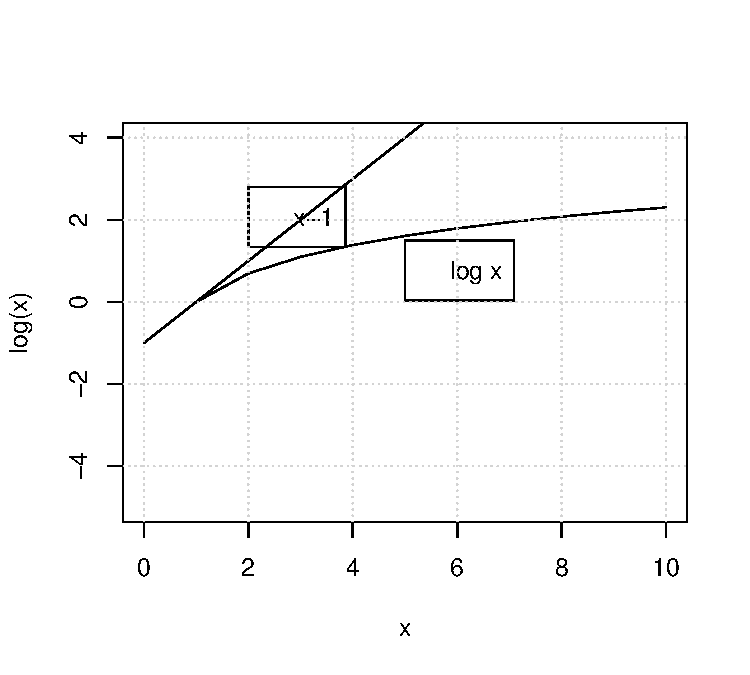
\includegraphics[width=\maxwidth]{figure/plot1-1} 

}



\end{knitrout}

as $n\rightarrow \infty$, provided that $a_nx+b_n\xrightarrow{n\rightarrow\infty}\infty$ where
$a_1,a_2,...>0$ and $b_1,b_2,...\in\mathbb{R}$. Let us consider $F(x)=1-x^{-\alpha}\ \ \forall x \geq 1$ and $b_1=b_2=...=0$.

$$n\{1-F(a_nx)\}=n(a_nx)^{-\alpha}=x^{-\alpha}$$
would give us 
$$log P[\frac{M_n}{a_n}\leq x]\xrightarrow{n\rightarrow\infty}\exp\{-x^{-\alpha}\}$$
<=>
$$P[\frac{M_n}{a_n}\leq x]\xrightarrow{n\rightarrow\infty}\exp\{-x^{-\alpha}\}$$
$$\frac{M_n}{a_n}\xrightarrow{d} Fréchet(\alpha)$$
$$na_n^{-\alpha}=1<=>a_n^{-\alpha}=n^{-1}<=>a_n=n^{1/\alpha}$$
Thus $n^{1/\alpha}M_n\xrightarrow{d}Frechet(\alpha)$ as  can be expressed in terms of $F$ as follows.

$$1-x^{-\alpha}=u<=>x=(1-u)^{-1/\alpha}$$
$$F^{(-1)}(u)=(1-u)^{-1/\alpha}$$
$$F^{-1}(1-\frac{1}{n})=(1-\{1-\frac{1}{n}\})^{-\frac{1}{\alpha}}=(\frac{1}{n})^{-\frac{1}{\alpha}}$$
$$=n^{\frac{1}{\alpha}}=a_n$$

Thus $1-\frac{1}{n}=F(a_n)<=>$ $$\frac{1}{n}<=>1-F(a_n)<=>n=\{1-F(a_n)\}^{-1}$$

Let us keep this relation  for a more general distribution function $F$.

Thus
$$n\{1-F(a_nx)\}=\frac{1-F(a_nx)}{1-F(a_n)}$$
$$\xrightarrow{n\rightarrow\infty}x^{-\alpha}$$
if $F$ is of Pareto-type.

Therefore, from the previous computations
$$M_n\xrightarrow{d} Fréchet (\alpha)$$
where $a_n=F^{(-1)}(1-\frac{1}{n})$


This result is the Fréchet limit theorem for maxima, when the individual losses are of Pareto-type, then the sample  maximum is asymptotically Fréchet.

Some computations

$$\lim_{x\rightarrow\infty}\frac{\log(tx)}{\log x}=\lim_{x\rightarrow\infty}\frac{\log t}{\log x}+\frac{\log x}{\log x}=1\ \ \log \in R_0$$


$$\log^{(0)}x=x, \log^{(1)}=\log x$$
$\log^{(k)}=\log \log^{(k-1)}x$ for $k=1,2,\ldots$

$$\lim_{x\rightarrow\infty}\frac{log^{(k)tx}}{log^{(k)}x}
=\lim_{x\rightarrow\infty}\frac{\frac{t}{log^{(k-1)}tx...log tx tx}}{\frac{1}{log^{(k-1)}x...log x x}}=1$$
Then $log^{(k)}\in R_0$

\section{Thursday 16/03/17}
\section{Pareto Type Distributions}
\begin{defi}
$F$ is of Pareto type if $1-F\in\mathbb{R}_{-\alpha}$ for some $\alpha>0$. Remember that $(f\in\mathbb{R}_{\delta),\delta\in\mathbb{R}$ if $\frac{f(tx)}{f(x)}\xrightarrow{t^{\delta}}$.
Thus $1-F(x)=x^{-\alpha}l(x)$ where $l\in\mathbb{R_0}$.
\end{defi}

Some examples\\
\begin{exm}Pareto\\
\begin{align*}
F(x)&=1-x^{-\alpha}\forall x >1\\
F(x)&=x^{-\alpha}.1 (l(x)=1)\\
\end{align*}
\end{exm}

\begin{exm}Burr\\
F(x)=1-\left(\frac{\beta}{\beta+x^{\tau}}\right)^{\lambda}, \forall x>0\ \beta\lambda\tau>0\\
\begin{align*}
\lim_{x\rightarrow\infty}\frac{1-F(tx)}{1-F(x)}}&=(\lim_{x\rightarrow \infty}\frac{\beta+x^{\tau}}{\beta+(tx)^{\tau}}\)^{\lambda}\\
&=(t^{-\tau})^{\lambda}=t^{-\lambda\tau}\\
\end{align*}
\text{ Thus } -\alpha=\lambda\tau \text{( is the index of regular variation )}\\
l(x)=x^{\lambda\tau}(\frac{\beta}{\beta+x^{\tau}})^{\lambda}=(\frac{\beta x^{\tau}}{\beta+x^{\tau}})^{\lambda}\\
\end{exm}

\begin{exm}Fréchet\\
F(x)=exp\{-x^{-\alpha}\}\ \ \forall x>0,\alpha>0\\
\begin{align*}
\lim_{x\rightarrow{\infty}}\frac{1-F(tx)}{1-F(x)}&=\lim_{x\rightarrow\infty}\frac{1-exp\{-(tx)^{-\alpha}\}}{1-exp^{-x^{-\alpha}}}\\

&=\lim_{x\rightarrow\infty}\frac{\alpha(tx)^{-\alpha-1}t \ exp \{-(tx)^{-\alpha}\}}{\alpha x^{-\alpha-1}exp\{-x^{-\alpha}\}}\\
&=t^{-\alpha}\\

1-F(x)&=x^{-\alpha}l(x)$ \text{ where } $l(x)=x^{\alpha}(1-exp\{-x^{-\alpha}\})\\
      &=x^{\alpha}(1-exp\{-x^{-\alpha}\})\\
&=x^{\alpha}(1-[1-x^{-\alpha}+\frac{1}{2}x^{-2\alpha}-\frac{1}{3!}x^{-3\alpha}+...])\\
&=1-\frac{1}{2}x^{-\alpha}+\frac{1}{3!}x^{-2\alpha}+...\\
\end{align*}
\end{exm}

\begin{thm}Karamata\\



%30-03-2017
%Measures of Risk
\begin{defi}
$\rho:L_p(\Omega\rightarrow\mathbb{R}^+)$, is a measure of risk coherent. It hass the next properties:
\begin{itemize}
\item \rho(X+Y)\leq \rho(X)+\rho(Y)
\item X\leq Y a.s \Rightarrow \rho(X)\leq \rho(Y)
\item \rho(cX)=c\rho(X), \forall c>0
\item \rho(c+X)=c+\rho(X), \forall c>0
\end{itemize}
\end{defi}
Interpretations:\\
(1) Aggregation of risks is beneficial\\
(3) Scale invariance (e.g for change of currency) $X=0 a.s \Rightarrow \rho(0)=0$ \\
(4) $X=0 a.s\Rightarrow \rho(c)=c+\rho(0)$\\
                        $\Rightarrow \rho(c)=c $ from (3)\\
                        
\begin{exm} Standard Deviation Principle\\
$\rho(X)=\mu_x+K\sigma_x$ for some $k>0$, where $\mu_x=E[X]$ and $\sigma_x=var(X)$\\
(1) $\rho(X+Y)=\mu_x+\mu_y+k(\sigma^2_x+\sigma^2_y+2\sigma_{xy})$, where $\mu_Y=E[Y]$, $\sigma^2_Y=var(Y)$ and $\sigma_{XY}=cov(X,Y)$\\

$\rho(X)+\rho(Y)=\mu_x+\mu_y+k(\sigma_x+\sigma_y)$\\
$\rho(X+Y)\leq \rho(X)+\rho(Y)\Leftrightarrow$\\
$(\sigma^2_X+\sigma^2_Y+2\sigma_{XY})^{1/2}\leq \sigma_x+\sigma_Y\Leftrightarrow$\\
$\sigma^2_X+\sigma^2_Y+2\sigma_{XY}\leq \sigma_x+\sigma_Y+2\sigma_X\sigma_Y\Leftrightarrow$\\
$\sigma_{XY}\leq \sigma_X\sigma_Y$\\
Which is true from the Cauchy Schwarz inequality

We  can easily show that (3) and (4) hold also 
\begin{knitrout}
\definecolor{shadecolor}{rgb}{0.969, 0.969, 0.969}\color{fgcolor}\begin{kframe}


{\ttfamily\noindent\bfseries\color{errorcolor}{\#\# Error in xy.coords(x, y): 'x' and 'y' lengths differ}}\end{kframe}

{\centering 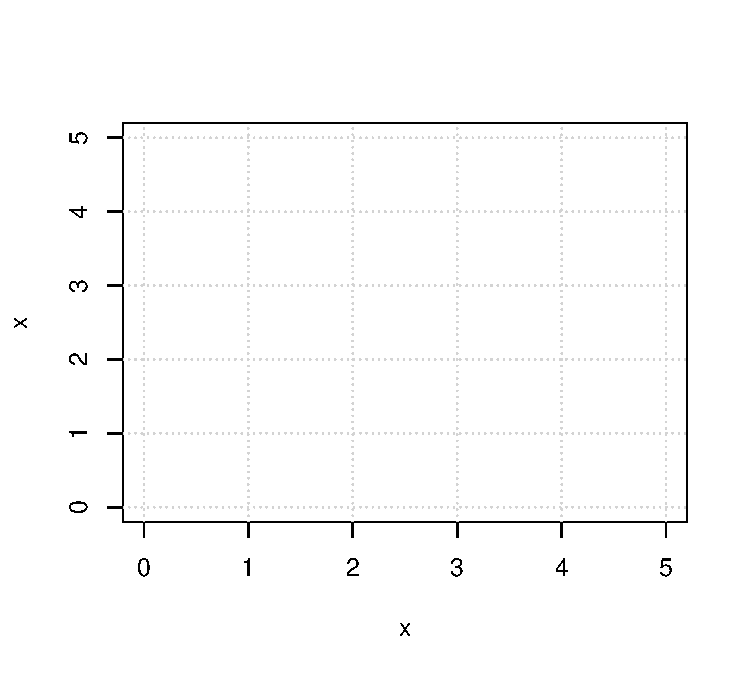
\includegraphics[width=\maxwidth]{figure/33-1} 

}



\end{knitrout}

$\mu_x=0\times 0.025+4\times0.75=3$\\
$E[X^2]=0^2\times0.025+4^2\times 0.75=12$\\
$\sigma^2_X=12-3^2=3$\\
$\mu_Y=4,\sigma_Y=0$\\
Let $k=1$, then $\rho(X)\leq\rho(Y)\Leftrightarrow 3+\sqrt(3)\leq 4\Leftrightarrow \sqrt(3)\leq 1$ which is false.
\end{exm}
                        
\begin{defi} The $\alpha-th$ value-at-risk $(VaR)$ is the $\alpha-th$ quantile of the distribution of the loss $X$, $\forall \alpha\in(0,1)$\\

The $\alpha -th$ quantile of the d.f F is any value $q_{\alpha}$\in\mathbb{R}$ s.t $\forall\alpha\in(0,1)$

\begin{itemize}
\item $F(X)\leq \alpha,\forall x<q_{\alpha}$
\item $F(x)\geq \alpha \forall x>q_{\alpha}$
\end{itemize}
\end{defi}

If $q_{\alpha}$ is not unique, one can choose for example:
$$q_{\alpha}=F^{-1}(\alpha)=inf\{x\in\mathbb{R}|F(x)\geq \alpha\}$$


Note that $(*)$ can be re-expressed as $F(q_{\alpha^-})\leq \alpha$ and $F(q_{\alpha})\geq \alpha$ because $F(q_{\alpha+})=F(q_{\alpha})$.\\
The $Var$ is unfortunately not subadditive.\\
Let $Z$ have d.f $F_Z$ (strictly) increasing and continuous with $F_z(1)=0.91$  $F_z(90)=0.95$ and $F_z(100)=0.96$\\

%plot2


Let $X=ZI\{Z\leq 100\}$ and  $Y=ZI\{Z\geq 100\}$. So $X+Y=Z(I\{Z\leq 100\}+\{Z>100\})=Z$\\

\begin{align*}
F_x(1)&=P[X\leq 1|Z\leq 100]P[Z\leq 100]+ P[X\leq 1|Z>100]P[Z>100]\\
&=P[Z\leq 1]+P[Z>100]=0.91+0.04=0.95
\end{align}
Let us check that $F_x(x)$ is continuous at $x=1$ for $\delta$ sufficiently close to zero.

\begin{align*}
F_x(1+\delta)&=P[Z\leq 1+\delta]+ P[Z> 100]\\
&=F_z(1+\delta)+0.04
\end{align}
and so $F_x$ is strictly increasing and continuous at $1$.\\

Defining $VaR_{\alpha}(U)$ as the $\alpha-th$ quantile of the random loss $U$, we have $VaR_{0.95}(X)=1$

\begin{align*}
F_Y(0)&=P[Y\leq 0]\\
&=P[Y\leq 0|Z\leq 100]P[Z\leq 100]+P[Y\leq 0|Z>100]P[Z>100]\\
&=P[Z>\geq 100]+P[Z\leq 0|Z>100]P[Z>100]=0.96
\end{align*}
Thus $VaR_{0.95}(Y)\geq 0$ and so $VaR_{0.95}+VaR0.95(Y)\leq 1<90VaR_{0.95}(X+Y)$\\
  
  \begin{defi}
  The $\alpha-th$ tile value at risk $(TVaR)$ of the random loss is:
  $$TVaR_{\alpha}=E[X|X>q_{\alpha}],$$
  where q_{\alpha} is the $\alpha-th$ quantile or $VaR$ of $X$, $\forall \alpha\in(0,1)$
  \end{defi}
 The TVaR makes good use of the information of the tail of the loss distribution and it is coherent.\\
 If the d.f of $X$ $F_X$ is continuous at $q_{\alpha}$ then 
 
 \begin{align*}
 TVaR_{\alpha}(X)&=\frac{\int_{q_{\alpha}}^{\infty}xdF_x(x)}{1-F_x(q_{\alpha})}\\
 &=\frac{\int_{q_{\alpha}}^{\infty}xdF_x(x)}{1-\alpha}
  \end{align*}
If $F_x$ is continuous and stricctly increasing, then:
\begin{align*}
\int_{q_{\alpha}}^{\infty}xdF_x(x)&=\int_{\alpha}^1 F_x^(-1)(u)du\\
&=\int_{\alpha}^1 VaR_u(X)du\ \ \ \ (F_x(x)=u,x=F_x^{(-1)}(u))\\
Thus \ \ \ TVaR_{\alpha}(X)&=\frac{\int_{\alpha}^{1}VaR_u(X)}{1-\alpha}
\end{align*}
which is the average of $VaR_u$ for $u\in[\alpha,1)$
$$TVaR(X)=ex(q_{\alpha})+q_{\alpha}$$
\begin{exm}X\sim Exponential(\theta)\\
$F(x)=1-e^{-\theta x}=u\Leftrightarrow -\frac{1}{\theta}log(1-u)=x$\\
so\\
$VaR_{\alpha(X)=q_{\alpha}=-\frac{1}{\theta}log(1-\alpha)$\\
$ex(a)=E[X]=\frac{1}{\theta}$, $\forall a\geq 0$\\
$TVaR_{\alpha}(X)=\frac{1}{\theta}-\frac{1}{\theta}log(1-\alpha)=\frac{1}{\theta}\{1-log(1-\alpha)\}$
\end{exm}


\begin{exm}X\sim\cal{N(\mu,\sigma^2)}\\
$VaR_{\alpha(X)}=\mu+\sigma\Phi ^{(-1)}(\alpha)$ ,\ where $\Phi$ is the d.f of $\cal{N}(0,1)$\\
If $\Phi=\Phi^{'},$ then\\

\int_{\alpha}^{\infty}x\Phi(x)dx=-\int_{a}^{\infty}\Phi^{'}(x)dx=-[0-\Phi(a)]=\Phi(a)\\
\end{exm}

$X$ has density $\frac{1}{\sigma}\Phi(\frac{x-\mu}{\sigma})$\\

\begin{align*}
TVaR_{\alpha}(X)&=\frac{\int_{q_{\alpha}}^{\infty}x\frac{1}{\sigma}\Phi(\frac{x-\mu}{\sigma})dx}{1-\alpha}\\
&=\frac{1}{1-\alpha}\int_{\frac{q_{\alpha}-\mu}{\sigma}}^{\infty}(\mu+\sigma y)\frac{1}{\sigma}\phi(y)\sigma dy \ \ \ \ (y=\frac{x-\mu}{\sigma}, \mu+\sigma y=x)\\
&=\frac{1}{1-\alpha}\{\mu[1-\phi\circ \phi^{-1}(\alpha)]+\sigma\int_{\phi^{(-1)}(\alpha)}^{\infty}y\phi(y)dy\}\\
&=\frac{1}{1-\alpha}\{\mu(1-\alpha)+\sigma\phi\phi^{(-1)(\alpha)}\}\\
&=\mu+\frac{\sigma}{1-\alpha} \phi\circ\phi^{-1}(\alpha)
\end{align*}



%Thursday 06/04/2017

\section{Birth Processes}
$$p_{k,k+n}(s,t)=P[N_t-N_s=n|N_s=k]$$
transition probability
$$p_{k,k+n}(t,t+h)=	\left\{
		\begin{array}{ll}
			1-\lambda_k(t)+o(h)&if n=0 \\
			\lambda_k(t)h+o(h)&if n=1 \\
	    o(h) & if n=2,3,...
		\end{array}
	\right.
$$
\begin{thm}
The transition probabilities $\{p_{k,k+n}(s,t)\}$ of the non homogeneus birth process are $\forall 0\leq s<t,K\geq 0$ and $n\geq 1$,
$$p_{k,k}(s,t)=exp\{-\displaystyle\int_s^t\lambda_k(x)dx\}$$ and 
$$p_{k,k+n}(s,t)=\displaystyle\int_{s}^t \lambda_{k+n-1}(y)p_{k,k+n-1}(s,y)exp\{-\displaystyle\int_{y}^t\lambda_{k+n}(x)dx\}dy$$
\end{thm}


A sufficient condition for $\displaystyle\sum_{n=0}^{\infty}p_{k,k+n}(s,t)=1$ $\forall 0\leq s <t$, $k\geq 0$ is $$\displaystyle\sum_{k=0}^{\infty}\frac{1}{\displaystyle\max_{t\geq 0}\lambda_k(t)}=\infty$$

\begin{coro}
The homogeneus Poisson process, which is obtained by $\lambda_0(t)=\lambda_1(t)=...=\lambda>0$ has transition probabilities $$p_{k,k+n}(s,t)=e^{-\lambda(t-s)}\frac{\{\lambda(t-s)\}^n}{n!}\ \ \ \forall 0\leqs>t,k,n\geq 0$$
\end{coro}

\begin{proof}
This is clear for $n=0$.\\
Assume the formula true for $n-1$, then 
\begin{align*}
p_{k,k+n}(s,t)&=\displaystyle\int_{s}^t\lambda e^{-\lambda(y-s)}\frac{\{\lambda(y-s)\}^{n-1}}{(n-1)!}exp\{-\displaystyle\int_y^t\lambda dx\}dy\\
&=\displaystyle\int_s^t\lambda^ne^{-\lambda(y-s)-\lambda(t-y)}\frac{(y-s)^{n-1}}{(n-1)!}dy\\
&=\frac{\lambda^n e^{-\lambda(t-s)}}{(n-1)!}\int_{s}^t(y-s)^{n-1}dy\\
&=e^{-\lambda(t-s)}\frac{\{\lambda(t-s)^n\}}{n!}\\
\end{align*}
\end{proof}

\begin{coro}
The non homogeneus Poisson process, which is obtained by $\lambda_0(t)$=\lambda_1(t)=...=\lambda(t)$ has transition probabilities $$p_{k,k+n}(s,t)=exp\{-\displaystyle\int_s^t\lambda(x)dx\}\frac{\{\displaystyle\int_s^t\lambda(x)dx\}^n}{n!} \ \ \ \forall 0\leq s<t,\ k,n\geq 0$$
\end{coro}

One can for example compute the expected number of claims during (s,t) as $\int_s^t\lambda(x)dx$. The increments are no longer stationary but still independent.\\
Birth processes with contagion can be used when the increments are desired dependent. We consider
$$\lambda_k(t)=\alpha+\beta k\ \ \ with \ \ \alpha>0$$
$\beta\neq 0 $ satisfies $\alpha+\beta k\geq 0\ \ \ for \ \ k=0,1,...$

These processes are homogeneus.
\begin{coro} THe transition probability of a contagious birth process are given by:
$$p_{k,k+n}(s,t)=\binom{\frac{\alpha}{\beta}+k+n-1}{n}e^{-(\alpha+\beta k)(t-s)}$$
$$\{1-e^{-\beta(t-s)}\}^n$$
\end{coro}

\begin{knitrout}
\definecolor{shadecolor}{rgb}{0.969, 0.969, 0.969}\color{fgcolor}

{\centering 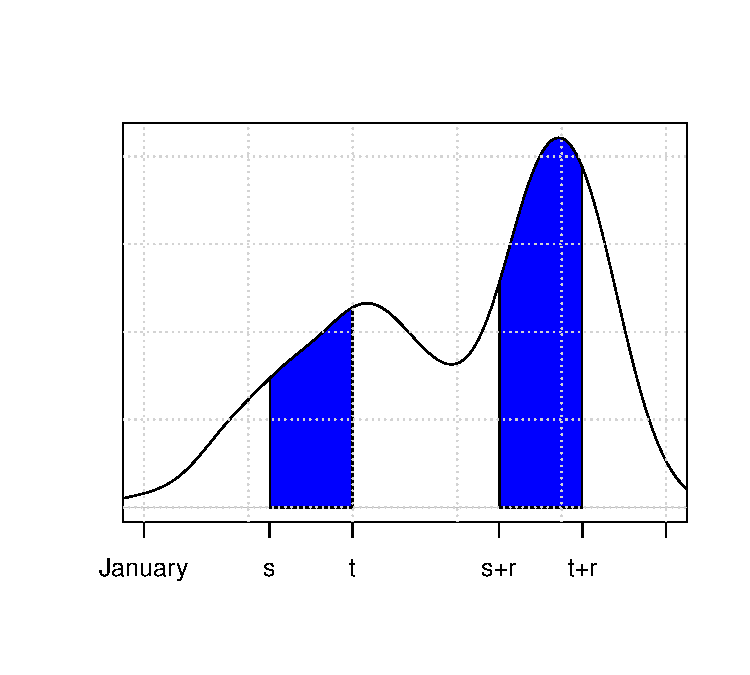
\includegraphics[width=\maxwidth]{figure/06/4-1} 

}



\end{knitrout}

Reminder $$\binom{x}{k}=\left\{\begin{array}{ll}
\frac{[x]_k}{k!}& if k=1,2,..\\
1&if k=0\\
0, &if k=-1,-2,...
\end{array}
$$
$$[x]_k=x(x-1)...(x-k-1)$$
$$\binom{x-1}{n}=\frac{n+1}{x}\binom{x}{n+1}$$
When $n=0$ $p_{k,k(s,t)=e^{(\alpha+\beta k)(t-s)}}$, assume the formula true for $n$, then:
\begin{align*}
p_{k,k+n+1}(s,t)&=\int_s^t\{\alpha+\beta(k+n)\}\binom{\frac{\alpha}{\beta}+k+n-1}{n}e^{-(\alpha+\beta k)(y-s)}\{1-e^{-\beta(y-s)}\}^n\\
&=\binom{\frac{\alpha}{\beta}+k+n}{n+1}\frac{n+1}{\frac{\alpha}{\beta}+k+n}\{\alpha+\beta(k+n)\}e^{
-(\alpha+\beta k)(y-s)}e^{-(\alpha+\beta k)(t-y)}\\
&=\binom{\frac{\alpha}{\beta}+k+n}{n+1}\beta(n+1)e^{-(\alha+\beta k)(t-s)}\int_s^t\{e^{-\beta(t-y)}-e^{-\beta(t-s)}\}^ne^{-\beta(t-y)}dy\\
.......
\end{align*}



%27/04/2017
\begin{section}{Risk Process}
The following quantities are required to define the risk process $X_1,X_2,...$ are independent individual losses or claim amounts (non-negativa r.v) with distribution function $F$ and expectation $\mu$ finite.\\
 $K_t$ is the number of individual claims occuring during $[0,t]\ \forall t\geq 0$.\\
 $\{K_t\}_{t\geq 0}$ is a birth process independent of $\{X\}]_{k\geq 1}$.\\
 The total loss or claim amount is $Z_t=\displaystyle\sum_{k=0}^{K_t}X_k$ where $X_0=0$.\\
 Let $r_o\geq 0$ be the initial capital of the insurance and $c>0$ be the premium rate (assumed constant), the $$Y_t=r_0+ct-Z_t,\forall t\geq 0$$ is the risk process.
 
 %falta plot%
 
 Let $T_k$ be the time of the k-th claim, thus.
 $$T_k=inf\{t\geq 0|K_t\geq k\}$$
 for $k=0,1,...$\\
 Let $D_k=T_k-T_{k-1}$ for $k=1,2,...$ be the interclaim times.\\
 If $D_1,D_2,...$ are i.i.d, then $\{T_k\}_{k\geq 0}$ or $\{K_t\}_{t\geq 0}$ are called renewal processes.\\
 
 For example, if $\{K_t\}_{t\geq 0}$ is the homogeneous Poisson process with rate $\lambda>0$, the $D_1,D_2,...$ are independent exponential $(\lamda)$, $(\lambda e^{-\lambda x})$ is the density.\\
 We focus on renewal conting process. In this case we define 
 $$\rho=\frac{E[X_1]}{E[D_1]}$$
 For the Poisson process 
 \begin{align*}
 E[D_1]&=\frac{1}{\lambda}\int_0^{\infty}x\lambda e^{-\lambda x}d(x\lambda)\\
 &=\frac{1}{\lambda}\Gamma(2)\\
 &=\frac{1}{\lambda}
 \end{align*}
 
 $\rho=\frac{E[X_1]}{E[D_1]}=\lambda\mu$, we define the \textbf{security loading} (Siche heitszuschlag)$$\beta=\frac{c-\rho}{\rho}$$.
 
 Let $t^{\dagger}$ be any time horizon, then $$\Psi(r_0,t^{\dagger})=P[inf_{0\leq t\leq t^{\dagger}}Y_t<0]$$ is the probability of ruin in the finite time horizon $[0,t^{\dagger}]$
 \begin{align*}
 \psi(r_o)&=\lim_{t^{\dagger}\rightarrow\infty}\psi(r_0,t^{\dagger})\\
          &=P[inf_{0\leq t \leq \infty}Y_t<0]\\
 \end{align*}
 Is the probability of ruin in infinite time horizon or simply the probability of ruin. We define the time of first ruin as 
 
$T=\left\{\begin{array}{ll}
inf\{t\geq 0|Y_t<0\}& if the infimum is finitek\\
\infty&otherwise\\
\end{array}
$$
 Thus $\psi(r_0,t^{\dagger})=P[T\leq t^{\dagger}]\xrightarrow{t^{\dagger}\rightarrow\infty}\psi(r_0)$
 
 %falta plot
 
 $\psi(r_0)<1\Rightarrow T$ has a defective distribution.\\
 Some possible generalization of the basic risk procecss (of Lundberg). A Wiener Process is a stochastic process $\{W_t\}_{t\geq 0}$ with $W_0=0$ a.s, with continuous sample paths a.s, with independent increments and with $W_t-W_s\sim N(0,t-s)\ \ \ \forall 0\leq s < t < \infty$
 
 %falta grafico de wiener process%
 It is tiically used to add noise to a stochastic process.
 $$Y_t=r_0+cct-Z_t+\sigma W_t \ \ \forall t \geq 0$$ perturbed risk process.
 $$Y_t=r_0+ct-Z_t+\int_{0}^tY_sds,$$ where $r$ is the fixed interest rate.

$$Y_t=r_0+ct-Z_t+\int_0^tY_sdR_s\ \forall t\geq 0$$ where $\{R_t\}$ is the stochastic process of the interest rates ($R_s=r$ gives the previous case).
We can also consider the inhomogeneous Poisson process.

\begin{thm}Consider the renewal risk process, then $\beta<0\Rightarrow\psi(r_0)=1$
\end{thm}
\begin{proof}
FOr $n=1,2,...,$ 
\begin{align*}
Y_{T_n}&=r_0+cT_n-Z_{T_n}\\
&=r_0+c\displasystyle\sum_{k=1}^{n}D_k-\displaystyle\sum_{k=1}^{K_{T_n}}X_k\\
&=r_0+\displaystyle\sym_{k=1}^{n}V_k,\ \text{where}\\
V_k&=cD_k-X_k, for k=1,2,...\\
\frac{Y_{T_n}}{n}\xrightarrow{a.s} E[V_1]\\
\end{align*}
from the strong law of large numbers 
$$Y_{T_n}\xrightarrow{a.s}sgnE[V_1].\infty$$.
\begin{align*}
\beta<0&\Leftrightarrow c<\rho\\
&\Leftrightarrow c<\frac{E[X_1]}{E[D_1]}\\
&\Leftrightarrow c E[D_1]-E[X_1]<0\\
&\Leftrightarrow E[V_1]<0\\
\end{align*}

Thus $Y_{T_n}\xrightarrow{a.s}-\infty$, which means that $\{Y_t\}_{t\geq 0}$ downcrosses the null line a.s, viz $\psi(r_0=1)$.
\end{proof}

Note that $E[D_1]<\infty$ is an assumption of the definition ot the renewal process.\\
We will now show in detail that in compound Poisson risk process $\frac{Z_t}{t}\xrightarrow{a.s}\rho \ \ (as t\rightarrow \infty)$ and $\psi(r_0)=1$, if $\beta\leq 0$.\\

We define the loss process as $L_t=Z_t-ct\ \ \forall t\geq 0$

\begin{lema}
Let n\in\{0,1,...\}, h>0, t\in[nh,(n+1)h], then L_{nh}-h\leq L_t\leq L_{(n+1)+h}
\end{lema}
\begin{proof}
Let r,s>0
\begin{align*}
L_{r+s}-L_r&=Z_{r+s}-(r+s)-Z_r+r\\
&=\underbrace{Z_{r+s}-Z_r}_{\geq 0}-s\\
&=0\\
\end{align*}
When no claims occur during $[r,r+s]$ In this case, $L_{r+s}-L_r=-s$ viz $L_{r+s}\geq L_r-s$ . For $r=nh$, $t=r+s=nh+s$ and $s\in[0,h],$ we have $L_t\geq L_{nh}-s\geq L_{nh}-h$. The upper bound can be shown in the same way.
\end{proof}

\begin{thm}
1.- $\frac{L_t}{t}\xrightarrow{a.s}\rho-1, \ \ \forall \beta\in\mathbb{R}$\\
2.- L_t\xrightarrow\infty, \ if \  \beta<0\\
3.- L_t\xirghtarrow{as}-\infty,\ \ if \beta>0\\
4.- liminf_{t\rightarrow \infty} L_t=-\infty \ \ a.s \ \ and \ \ limsup_{t\rightarrow\infty}L_t=\infty \ \ a.s., \ \ if \ \ \beta=0\\ 
\end{thm}
\begin{proof}
Let $h>0$, then $\{L_{nh}\}_{n\geq 0}$ is a random walk $(L_h,L_{2h}-L_h,L_{3h}-L_{2h},...)$ are i.i.d, which follows from the fact that $\{K_t\}_{t\geq 0}$ has stationary and independent increments and $X_1,X_2,...$ are independent.
From the strong law of large numbers

\begin{align*}
\frac{L_{nh}}{n}\xrightarrow{as}E[L_h]&=E[Z_h]-h\\
&=\lambda h \mu-h=h(\rho-1)\\
 liminf_{t\rightarrow\infty}\frac{L_t}{t}&=\lim_{n\rightarrow\infty}inf_{t\geq nh}\frac{L_t}{t}\\
&=\lim_{n\rightarrow\infty}inf_{k\geq n}\underbrace{inf_{kh\leq t\leq(k+1)h}\frac{L_t}{t}}_{\geq\frac{L_{kh}-h}{(k+1)h}}\\
&\geq \frac{1}{h}\lim_{n\rightarrow\infty} inf\frac{L_{nh}}{n}=\frac{1}{h}h(\rho-1)\\
&=\rho-1\\
\end{align*}

So $\rho-1\leq \lim inf_{t\rightarrow\infty}\frac{L_t}{t}$ and we can show in the same way that $limsup_{t\rightarrow\infty}\frac{L_t}{t}\leq \rho-1$. So (1) holds, (2) and (3) follow directly from (1), $L_t\xrightarrow{a.s}sgn(\rho-1)\infty$, (4) follows  from the result on random walks $liminf_{n\rightarrow\infty}L_{nh}=-\infty$ a.s and $limsup_{n\rightarrow\infty}=L_{nh}=\infty$ a.s (given that the summand have expectation 0)
\end{proof}


 \end{section}

%04/05/2017
\section{Risk Process}
$L_t=Z_t-ct,\ \ \forall t \geq 0,\ \ (loss \ \ process)$\\
$Y_t=r_0-L_t=r_0+ct-Z_t,\ \ \forall t\geq 0$
 risk or surplus process.\\
 
 $\rho=\frac{E[X_1]}{E[D_1]}$\\
 In the poisson case $\rho=\lambda\mu$ $\beta=\frac{c-\rho}{\rho}$\\ 
 Poisson case:\\
 $c=1$ w.l.o.g $L_{nh}-h\leq L_t\leq L_{(n+1)h}+h$
 \begin{itemize}
 \item (1)$\frac{L_t}{t}\xrightarrow{a.s}\rho-1$\\
 \item (2)$\beta<0\RightarrowL_t\xrightarrow{a.s}\infty$\\
 \item (3)$\beta<0\Rightarrow L_t \xrightarrow{a.s}-\infty$\\
 \item (4)$\beta=0\Rightarrow \Rightarrow liminf_{t\rightarrow\infty} L_t$ $limsup_{t\rightarrow\infty}L_t=\infty$ a.s
 \end{itemize}
 
 Let $S=sup_{t\geq 0} L_t$ is the maximal (aggregate loss) \\
 \begin{align*}
 \psi(r_0)&=P[\inf_{t\geq 0} Y_t< 0]\\
  R(r_0)&=1-\psi(r_0)=1-P[\inf_{t\geq 0} Y_t<0]\\
 &=P[\inf_{t\geq0} Y_t\geq 0]\\ 
  &=P[\inf_{t\geq 0} r_0-L_t\geq 0]\\
  &=P[\inf_{t\geq 0}-L_t\geq-r_0]\\
  &=P[-\sup_{t\geq 0}L_t\geq-r_0]\\
  &=P[S\leq r_0]\\
  L_0=0 &\Rightarrow \sup_{t\geq 0}L_t \geq 0\\
\text{Consequently}\\
R(0)&=P[S\leq 0]\\
&=P[S=0]\\
&>0 \text{iff}\\
\psi(0)<1\\
\end{align*}
Therefore, in most cases, the distribution of $S$ is a mixture of an absolutely continuos distribution over $(0,\infty)$ and the Dirac probability at $0$ 
%Plot%
\begin{coro}
Let $r_0\geq 0$, then $$\psi(r_0)=\left\{\begin{array}{ll}
=1& if \beta\leq 0\\
<1&if \beta>0\\
\end{array}
$$
\end{coro}
 \begin{proof}
 Let $\beta<0$, then by $(2)$ of the theorem $S=\infty$ a.s.\\
 $\psi(r_0)=1-R(r_0)=1-P[\infty\leq r_0]=1,\ \ \forall r_0\geq 0$. \\ Let $\beta=0,$ then by $(4)$ of the theorem $S\geq \limsup_{t\rightarrow\infty}L_t=\infty$ and so $\psi(r_0)=1,\ \ \forall r_0\geq 0$.\\
 Let $\beta>0$, then from $\psi(r_0)\leq \psi(0)$ it is sufficient to show  $\psi(0)<1$. By contradiction, assume $\psi(0)=P[S>0]=1$
 
 Then $\{L_t\}_{t\geq 0}$ upcrosses the null line a.s. and let $T_1$ denote the first upcrossing time.\\
 Consider $\{L_t\}_{t\geq T_1}$, which downcrosses the null line a.s., from (3) of the theorem, and let $S_1$ denote the first downcrossing time.\\
 THen $\{L_t\}_{t\geq S_1}$ upcrosses the null line a.s. and we can then define $T_2$ as before and iterate further in this way.\\
 So $\{L_t\}_{t\geq 0}$ crosses the null line infinitely many times, which contradicts $(3)$ of the theorem.
 \end{proof}
 
 \begin{thm} As $t\rightarrow\infty$ 
 $$U_t=t^{-\frac{1}{2}}\{L_t-t(\rho-1)\}\xrightarrow{d}\mathcal{N}(0,\lambda\mu_2),$$ where $\mu_2=E[X_1^2],$ assumed finite.
 \end{thm}
 \begin{proof}
 $\{L_t\}_{t\geq 0}$ is a Lévy process $\Rightarrow \{L_{nh}_{n\geq 0}\}$ for any $h>0,$ is a random walk.
 \begin{align*}
 E[L_h]&=E[Z_h]-1=\lambda\mu h-1.h\\
&=h(\rho-1)\\
Var(L_h)&=Var(Z_h)=h\lambda\mu_2\\
 \end{align*}
 Thus, from the Central Limit theorem $$\frac{U_{nh}}{\sqrt{\lambda\mu_2}}=\frac{L_{nh}-nh(\rho-1)}{\sqrt{nh\lambda\mu_2}}\xrightarrow{d}\mathcal{N}(0,1)$$ Thus the theoremholds for $t\in\{nh\}_{n\geq 0}$. Let $t_n\in[nh,(n+1)h],$ then from the Lemma $$R_n=t_n^{-\frac{1}{2}}\{L_{nh}-h-t_n(\rho-1)\}\leq U_{t_n}$$ and $$S_n=t_n^{-\frac{1}{2}}\{(L_{(n+1)h}+h)-t_n(\rho-1)\}\leq U_{t_n}$$
 
 We have again $R_n\xrightarrow{d}\mathcal{N}(0,\lambda\mu_2)$(*) and $S_n\xrightarrow{d}\mathcal{N}(0,\lambda\mu_2)$. Thus $\forall x\in\mathbb{R}$ 
 $$\underbrace{P[S_n\leq x]}_{\xrightarrow{n\rightarrow\infty}\phi(\frac{x}{\sqrt{\lambda\mu_2}})}\leq P[U_{t_n}\leq x]\leq \underbrace{P[R_n\leq x]}_{\xrightarrow{n\rightarrow\infty}\phi(\frac{x}{\sqrt{\lambda\mu_2}})}$$
 --------------
 Detail of (*)
 $$R_n=\underbrace{(\frac{nh}{t_n})^{\frac{1}{2}}}_{\xrightarrow{a.s}1}\underbrace{(nh)^{-\frac{1}{2}}\{L_{nh}-nh(\rho-1)\}}_{\xrightarrow{d}\mathcal{N}(0,\lambda\mu_2)}$$
 $$\underbrace{t_n^{-\frac{1}{2}}\{(nh-t_n)(\rho-1)\}}_{\xrightarrow{n\rightarrow \infty}0}$$
  \end{proof}
 \section{Derivation of the integro-differential equation for the probability of ruin}
 $$P[K_h=n]=\left\{\begin{array}{lll}
=1-\lambdan+o(h), & if &n=0\\
\lambda h + o(h), & if& n=1\\
o(h), &if & n=2,3,..,\\
\end{array}
$$as $h\rightarrow\infty$
Assume one claim in $[0,h]$
%%PLOT2 falta
$X_1>r_0\Rightarrow$ no ruin in $[0,h]$\\
 $X_1>r_o+ch\Rightarrow$ ruin certain in $[0,h]$\\
 $r_0\leq X_1 < r_0+ch\Rightarrow$ ruin certain in $[0,s(x)]$ and no ruin $[s(x),h]$, where $X_1=x$, Thus $s(x)=\frac{x-r_0}{h}$, $r_0+s(x)h=x$
 
 %%%%%11/05/2017
$\psi(r_0)=(1-\lambda h)\psi(r_0+ch)+\lambdah \{\int_0^{r_0}\psi(r_0+ch-x)dF(x)+\int_{r_0}^{r_0+h}[\int_0^{s(x)}1\lambda e^{-\lambda t}dt+\int_{s(x)}^h\psi(r_0+ct-x)\lambda e^{-\lambda t}dt]dF(x)+\int_{r_0+ch}^{\infty}1dF(x)\}+o(h)$\\
$\psi(r_0)-\psi(r_0+ch)=-\lambda h\{\psi(r_0+ch)-\int_0^{r_0}\psi(r_0+ch-x)dF(x)-\int_{r_0}^{r_0+ch}[...]dF(x)-[1-F(r_0+ch)]\}+o(h)\Rightarrow \psi'(r_0)=\frac{\lambda}{c}\{\psi(r_0)-\int_0^{r_0}\psi(r_0-x)dF(x)-[1-F(r_0)]\}$
\begin{thm}
The general solution of the linear homogeneous differential equation of the second order $$y''(x)+by'(x)+cy(x)=0$$ has the form $$y(x)=a_1e^{r_1x}+a_2e^{r_2x},$$ where $a_1,a_2\in\mathbb{R}$ and $r_1,r_2\in\mathbb{R}$ satisfy auxiliary equation $r^2+br+c=0$ when $r_1\neq r_2$. If $r_1=r_2$ is the solution of the auxiliary equation, then the solution has the form $$y(x)=(a_1x+a_2)e^{r_1x}$$ We can obtain $a_1$ and $a_2$ with two boundary conditions.
Let $R(r_0)=1-\psi(r_0)$ be the survival probability, viz. the probability of non ruin with initial capital $r_0$.\\
Thus 
\begin{align*}
-R'(r_0)&=\frac{\lambda}{c}\{1-R(r_0)-\int\{1-R(r_0-x)\}dF(x)-1+F(r_0)\}\\
&=\frac{\lambda}{c}\{-R(r_0)+\int_0^{r_0}R(r_0-x)dF(x)\}\\
\text{Thus} R'(r_0)&=\frac{\lambda}{c}\{R(r_0)-\int_0^{r_0}R(r_0-x)dF(x)\}\\
\end{align*}
\end{thm}
\begin{exm}Linear combination of exponentials individual claim amount distribution
$$f(x)=e^{-3x}+\frac{10}{3}e^{-5x},\forall x>0$$
\beta=\frac{4}{11}\\
\mu=\int_0^{\infty}f(x)dx=\frac{1}{3}\frac{1}{3}+\frac{2}{3}\frac{1}{5}=\frac{1}{3}\frac{5+6}{15}=\frac{11}{45}\\
...
\end{exm}
\section{Adjustment Coefficient}
 \begin{defi}The adjustment coefficient is the positive solution w.r.t $v$ of $$E[e^{vL_1}]=1$$ where $L_1=Z_{1-c}$ is the loss process at time $1$. It is denoted $r>0$
 \end{defi}
 Thus $E[e^{vZ_1}]e^{-vZ_1}=1$ viz . $$exp\{\lambda[M_x(v)-1]=e^{vc},\}$$ i.e
$$M_x(v)=1+\frac{c}{\lambda}v=1+(1+\beta)\mu v$$, where $M_x$ is the M.g.f of $X_1$ at $\mu$ its expectation.


\begin{exm}
\begin{align*}

f(x)&=\sqrt{\frac{\theta}{2\pi x^3}}exp\{-\frac{\theta}{2x}(\frac{x-\mu}{\mu})^2\}\\
\forall x>0, \text{ expectation }  \mu>0,\theta>0\\

M_x(v)&=\int_0^{\infty}e^{vx}f(x)dx\\
&=exp\{\frac{\theta}{\mu}[1-\sqrt{1-2\frac{\mu^2}{\theta}v}]\},\\
\forall v\leq \frac{1}{2}\frac{\theta}{\mu^2}
\end{align*}
\end{exm}

$M_x$ is not steep, so the adjustment coefficient may not exist, if $\beta$ is nor large enough.
\begin{thm}
In the compound Poisson risk process, if the adjustment coefficient $r$ exists, then, $\orall r_0\geq 0$
$$\psi(r_0)=\frac{e^{rr_0}}{E[exp\{-rY_T\}|T<\infty]}$$
\end{thm}
A simple proof of this result is based on the theory of martingales.
This formula is inappropiate for numerical evaluations.\\
\begin{coro}
Lundberg inequailtiy $$\forall r_0\geq 0,\psi(r_0)\leq e^{-rr_0}$$
\begin{proof}
This follows directly from $r>0$ and $Y_T<0$, then $\frac{\delta r}{\delta\beta}>0\Rightarrow \lim_{\beta\rightarrow 0,\beta>0} r=0\Rightarrow \lim_{\beta\rightarrow 0,\beta>0}\psi(r_0)=\lim_{r\rightarrow 0,r>0}\psi(r_0)=\lim_{r\rightarrow 0,r>0}\frac{e^{-rr_0}}{E[exp\{-rY_T|T<\infty\}]}=\frac{1}{1}=1$ (by monotone convergence.)\\
\end{proof}
\end{coro}
In the following case, the expectation of the last theorem can be evaluated.
\begin{exm}Erlang model
This is the compound Poisson risk process with $X_1\sim Exponential (\frac{1}{\mu})$
%%%Falta plot aqui

Let $C(r_0)=Y_{T-}$ is the surplus prior to ruin, defined over $\{T<\infty\}$ and let $X(r_0)$ be the claim amount leading to ruin. Thus $$-Y_T=X(r_0)-C(r_0)$$
Define $X\sim Exponential(\frac{1}{\mu})$ independent of $\{Z_t\}_{t\geq 0}$. Given $T<\infty$, $X(r_0)$ has some distribution as $X$ given $X>C(r_0)$ .
\end{exm}
 Let $y>0$, then 
 \begin{align*}
 P[Y_T<-y|T<\infty]&=P[X(r_0)-C(r_0)>y|T<\infty]\\
 &=P[X(r_0)-C(r_0)>y|T<\infty]\\
&=P[X(r_0>C(r_0)+y|T<\infty]\\
&=P[X>c(r_0)+y|X>C(r_0,T<\infty)]\\
&=P[X>y|T<\infty]\\
&=P[X>y|T<\infty]\\
&=P[X>y]=e^{-\frac{y}{\mu}},\forall y>0, 
\end{align*}
from the memoryless property of the exponential distribution 
\begin{align*}
E[exp\{-rY_T\}|T<\infty]=\int_0^{\infty}e^{ry}\frac{1}{\mu}e^{-\frac{y}{\mu}dy}\\
&=\frac{\frac{1}{\mu}}{\frac{1}{\mu}-r}(\frac{1}{\mu}-r)\int_0^{\infty}e^{-(\frac{1}{\mu}-r)y}dy\\
\end{align*}
$$=\frac{1}{1-\mu r}if $\frac{1}{\mu}-r>0$ }\Leftrightarrow $r<\frac{1}{\mu}$$ which holds because $\frac{1}{\mu}-\frac{\lambda}{c}(=\frac{\beta}{(1+\beta)\mu})$\\
$$\psi(r_0)=\frac{e^{-rr_0}}{\frac{1}{1-\mu r}}$$
$$\frac{e^{\frac{\beta}{(1+\beta)\mu}r_0}}{\frac{1}{1-\frac{\beta}{1+\beta}}}$$
$$\frac{e^{-\frac{\beta}{(1+\beta)\mu}r_0}}{1+\beta}$$

First result under initial capital

\begin{thm}
In the compound Poisson risk process with $r_0=0$ $\forall y\geq 0,$
$$P[Y_T<-y|T<\infty]\psi(o)=\frac{\lambda}{c}\int_y^{\infty}\{1-F(x)\}dx$$
This can be reformulated as $$P[-y-dy<Y_T<-y,T<\infty]=\frac{\lambda}{c}\{1-F(y)\}dy$$
We can consider any $r_0\geq 0 and define.
$$T_0=\left\{\begin{array}{ll}
=inf\{t\geq 0|Y_t<r_0\}& \text{ if the infimum is finite}\\
\infty &  \text{otherwise}\\
\end{array}$$
\end{thm}
i.e the first time that $\{\Y_t\}_{t\geq 0}$ goes below $r_0$\\
From shift invariance $$P[r_0-y-dy<T_{T_0}<r_0-y,T_0<\infty]=\frac{\lambda}{c}\int_0^{\infty}\{1-F(x)\}dx$$
$$\Leftrightarrow P[T<\infty]=\frac{\lambda\mu}{c}$$
$$\psi(0)=\frac{1}{1+\beta}$$

Let $R_1=r_0-Y_{T_0}=L_{T_0},$ over $\{T_0<\infty\},$ be the overshoot.\\
Let $y\geq 0$ the density of $R_1$ is 
\begin{align*}
f_R(y)dy&=P[y<R_1<y+dy|T_0<\infty]\\
&=P[y<r_0-Y_{T_0}<y+dy|T_0<\infty]\\
&=P[-r_0+y<-Y_{T_0}<-r_0+y+dy|T_0<\infty]\\
&=P[r_0-y-dy<Y_{T_0}<r_0-y|T_0<\infty]\\
&=\frac{\lambda}{c}\{1-F(y)\}dy\\
\end{align*}
\end{document}

 
